\part{Miscellaneous}
\chapter{Proofs}
\section{Induction}
\begin{defn}{Mathematical induction}{}
Let $P(n)$ be a family of statements indexed by $n \in \NN$.

By \vocab{mathematical induction}, If $P(0)$ is true and $P(k)$ is true $\forall k \in \NN$, then $P(n)$ is true $\forall n \in \NN$.\end{defn}

Steps to write the proof:
\begin{enumerate}
  \item \textbf{Base case.}
  
  Prove that $P(0)$ is true.
  \item \textbf{Inductive step.}.
  
  $P(k) \implies P(k+1)$
\end{enumerate}

\begin{exmp} Prove that \[ 1 + 2 + 3 + \cdots + n = \frac{n(n+1)}{2} \] for all positive integers $n$. \end{exmp}
\begin{proof} \ {\\}
The statement is true for $n=1$ (base case) because with $n=1$, LHS = RHS = $1$.

Assume that the statement is true for some $n=k$, where $k \in \ZZ^{+}$. By our induction hypothesis, we have $1 + 2 + 3 + \cdots + k = \dfrac{k(k+1)}{2}$.

To show that the statement is true for $k+1$, 
\begin{align*}
1 + 2 + 3 + \cdots + k + (k+1) &= \frac{k(k+1)}{2} + (k+1)\\
&= \frac{(k+1)(k+2)}{2}\\
&= \frac{(k+1)[(k+1)+1]}{2}
\end{align*}
$\because$ The statement holds true for $n=k$ and $n=k+1$, 

$\therefore$ The statement is true for all positive integers $n$. 
\end{proof}

\begin{defn}{Cauchy induction}{}
\vocab{Cauchy induction}, also known as forward-backward induction, is a variant of mathematical induction.
\end{defn}

To write the proof, there are a few steps:
\begin{enumerate}
  \item \textbf{Base case.}
  
  Prove that $P(0)$ is true.
  \item \textbf{Inductive step}.
  
  $P(k) \implies P(2k)$
  
  $P(k) \implies P(k-1)$
\end{enumerate}

\chapter{Calculus}
\section{Riemann Sums}
Given $y=f(x)$, we want to find the integral on the $x$-interval $[0,1]$.

Split the interval $[0,1]$ into $n$ equal subintervals \[ \left[0, \frac{1}{n}\right], \left[\frac{1}{n}, \frac{2}{n}\right], \cdots, \left[\frac{n-1}{n}, 1\right]. \]

\begin{figure}[H]
    \centering
    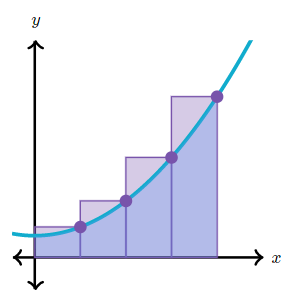
\includegraphics[width=6cm]{images/Riemanns_sums.png}
\end{figure}

Consider the height of the rectangles. We take the right value. Hence for the $k$-th subinterval $\sqbrac{\dfrac{k-1}{n}, \dfrac{k}{n}}$ where $k=1,\dots,n$, the height of rectangle is $f\left(\dfrac{k}{n}\right)$.\\

Area of $k$th rectangle is 
\[ \frac{1}{n} \cdot f\left(\frac{k}{n}\right).\]

Therefore, the integral is obtained by summing up the area of $n$ rectangles, which gives us
\begin{equation} 
\int_{0}^{1} f(x) \dd{x} = \lim_{n \to \infty} \sum_{k=1}^{n} \frac{1}{n} f\brac{\frac{k}{n}} 
\end{equation}
where there are infinitely many rectangles, i.e. $n \to \infty$.
\pagebreak

\section*{Problems}
\begin{prbm}[SMO 2020 Open Q10]
Find the value of 
\[ S = \lim_{n \to \infty} \sum_{k=1}^{n} \frac{1}{\sqrt{n(n+k)}} \]
\end{prbm}
    
\begin{solution}
\begin{align*}
S &= \lim_{n \to \infty} \sum_{k=1}^{n} \frac{1}{n} \sqrt{\frac{1}{1+\frac{k}{n}}}\\
&= \int_{0}^{1} \frac{1}{\sqrt{1+x}} \dd{x}\\
&= 2\sqrt{2} - 2
\end{align*}
\end{solution}

\begin{prbm}[SMO 2018 Open Q12]
Given that
\[ S=\lim_{n\to\infty}\sum_{k=1}^n\frac{1}{n+k} \]
Find the value of $S$.
\end{prbm}
\begin{solution}
Using Riemann sums,
\[ \lim_{n\to\infty}\sum_{k=1}^nf\brac{\frac{k}{n}} = \int_0^1f(x)\dd{x} \]
Hence
\[ S = \lim_{n\to\infty}\frac{1}{n}\sum_{k=1}^n\frac{1}{1+\frac{k}{n}} = \int_0^1\frac{1}{1+x}\dd{x} = \boxed{\ln2} \]
\end{solution}
